\chapter{需求分析}

本章主要对课程管理系统的需求进行分析,通过建立目标模型、用户用例模型、系统领域模型对系统的功能性需求以及非功能性需求进行准确的确定,明确系统的开发边界。

\section{目标模型}

目标模型是需求工程用于推导各级需求的关键模型,从任意一项目标出发向上推导更抽象、更概括的目标,向下推导更具体、更细致的需求。

\begin{figure}[!hbp]
  \begin{center}
    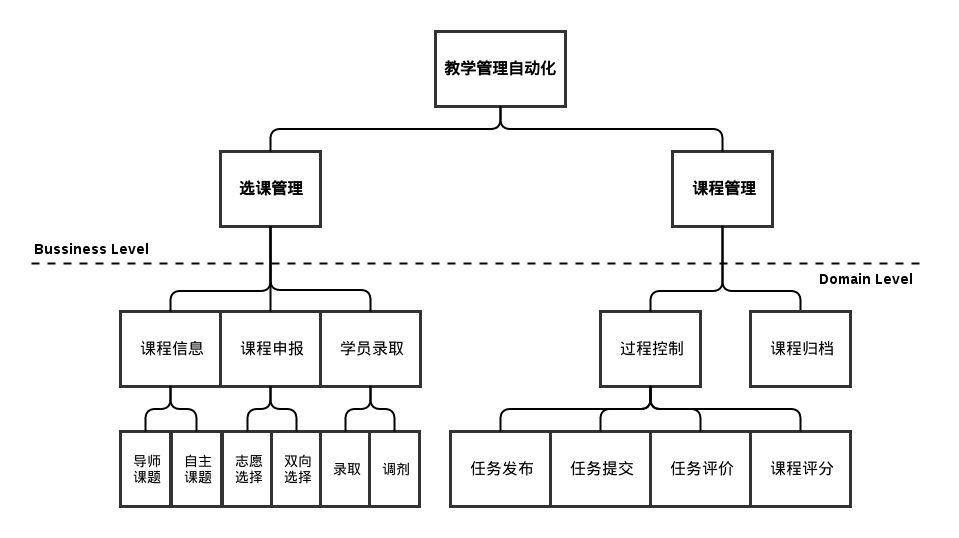
\includegraphics[scale=0.5]{figures/diagram-goal-model.png}
    \caption{目标模型示意图\label{GoalModel}}
  \end{center}
\end{figure}

图~\ref{GoalModel} 列出了系统业务目标和领域目标(需求)之间的层次关系。图中虚线所标识的位置是业务目标(Bussiness Goal)与领域目标的分界线,业务目标指的是在现实中实现这些业务所需要了解的目标; 领域目标指的是进行领域设计时需要了解的目标。将目标模型继续向下推导我们可以达到产品目标。

目标模型通过站在关系人(Stakeholder)的角度确定系统边界,系统目标可以通过对应关系直接转换为产品需求(\nameref{sec:appendix-requirement-table})

\section{用例模型}

在需求获取的过程中使用用例模型能够更清晰的与对方展开需求沟通。

\begin{figure}[!hbp]
  \begin{center}
    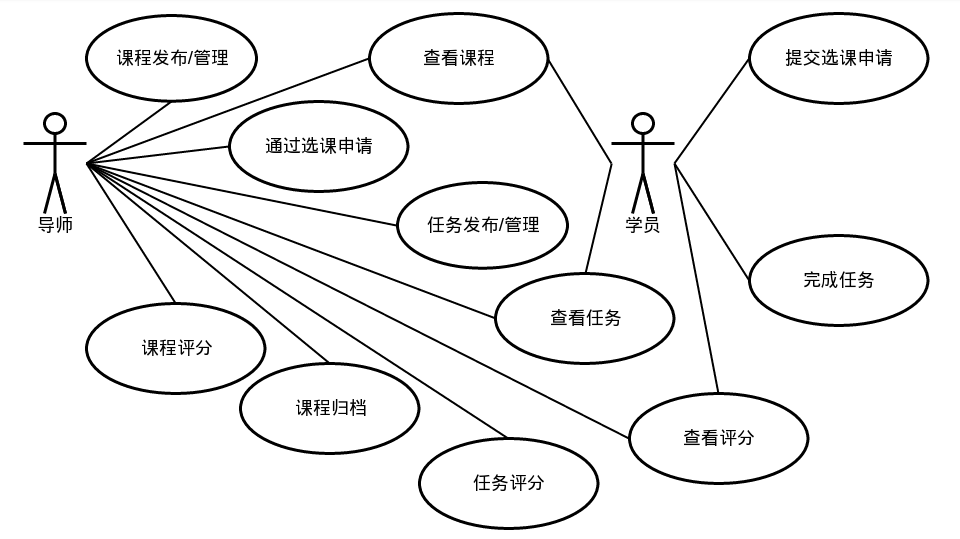
\includegraphics[scale=0.5]{figures/diagram-use-case.png}
    \caption{用户用例示意图\label{UseCase}}
  \end{center}
\end{figure}

图~\ref{UseCase} 所示的用户用例涉及多个交互,比较复杂,下文使用文本对不同的交互进行描述。可以看出课程管理系统的业务是导师与学员两类主要用户角色所主导的。

时间顺序上,每个课程拥有独立的过程控制点(阶段),系统根据课程所处的不同阶段对能对课程应用的业务操作进行控制和管理。

\subsection {交互: 发布课程}

用户使用导师身份进入系统后,执行下面的操作:

\begin{enumerate}
  \item 进入“发布课程”模块
  \item 填写课程标题、课程描述、授课规模以及其他自定义课程信息
  \item 提交课程信息
\end{enumerate}

课程信息提交后课程条目会出现在课程列表中,选择条目可以查看到导师填写的课程详细信息。

\subsection {交互: 选择课程与课程录取}

用户使用学员身份进入系统后,与系统进行下面的交互:

\begin{enumerate}
  \item 进入“课程申请”模块
  \item 选择课程列表中的课程条目
  \item 查看课程详细信息
  \item 提交课程申请
\end{enumerate}

提交课程申请之后还可以进行下面操作:

\begin{itemize}
  \item 撤销课程申请: 撤销已提交但未通过的课程申请
\end{itemize}

用户使用导师身份进入系统后,与系统进行下面的交互:

\begin{enumerate}
  \item 选择课程列表中的课程条目
  \item 进入课程详细信息
  \item 选择/取消课程申请列表中的学员条目
\end{enumerate}

还可以进行下面操作:

\begin{itemize}
  \item 录取结束: 完成所有录取操作(未来将不可增加/删除学员)
\end{itemize}

完成录取后,对应的课程就进入可以进行任务发布的状态。

\subsection {交互: 发布任务与完成任务}

用户使用导师身份进入系统后,与系统进行下面的交互:

\begin{enumerate}
  \item 选择课程列表中的课程条目
  \item 进入课程详细信息
  \item 选择“新任务”
  \item 输入任务所需的基本信息(标题、要求、截止时间)
  \item 提交任务信息
\end{enumerate}

用户使用学员身份进入系统后,与系统进行下面的交互:

\begin{enumerate}
  \item 选择课程列表中的课程条目
  \item 进入课程详细信息
  \item 选择未完成的任务条目
  \item 填写任务需要完成的项目(以在线表格或者文件上传等形式)
  \item 提交答案以完成任务
\end{enumerate}

完成任务后学员可继续提交、更新任务的答案直到导师做出任务评价。

\subsection {交互: 评价/评分}

用户使用导师身份进入系统后,与系统进行下面的交互:

\begin{enumerate}
  \item 选择课程列表中的课程条目
  \item 进入课程详细信息
  \item 进入课程学员列表
  \item 选择课程中的一位学员、查看任务列表
  \item 查看/下载学员提交的任务内容
  \item 填写任务评价/评分
  \item 提交评分表格
\end{enumerate}

在课程结束前,导师还会与系统进行下面的交互:

\begin{enumerate}
  \item 选择课程列表中的课程条目
  \item 进入课程详细信息
  \item 进入课程学员列表
  \item 选择课程中的一位学员、查看任务列表
  \item 填写该学员的课程评价/评分
  \item 提交评分表格
\end{enumerate}

导师完成课程评分后可在学员列表直接查看到学员的课程得分。 学员可在任务列表查看到导师发布的任务评价,在课程的详细信息页面查看到导师发布的课程评分。

\newpage

\section{系统领域模型}

建立系统领域模型可以帮助理解系统运行的外部环境以及系统开发的边界位置。

\begin{figure}[!hbp]
  \begin{center}
    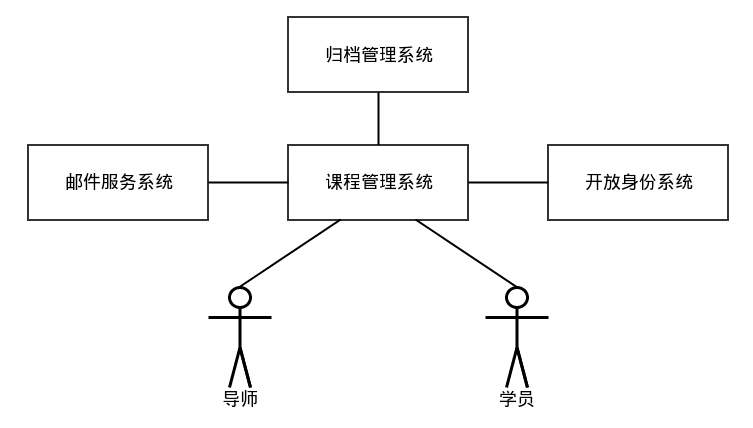
\includegraphics[scale=0.5]{figures/diagram-domain-model.png}
    \caption{领域模型示意图\label{DomainModel}}
  \end{center}
\end{figure}

图~\ref{DomainModel} 所示为系统的领域模型示意图,图中的系统分别负责:

\begin{itemize}
\item 用户身份系统,负责用户身份的验证,以便用户能在不同系统中使用同一个身份
\item 邮件服务系统,用于处理业务邮件请求(如发送通知、提醒)
\item 归档管理系统,管理来自不同系统的归档,提供归档和归档的索引及下载服务
\item 课程管理系统,本项目的目标系统,处理课程管理方面的业务请求
\end{itemize}

\subsection{业务过程模型}

作为面向业务产品领域的关键知识,项目对课程管理系统的业务过程建立了业务过程模型,使用图形化的语言简单清晰的描述了系统所需要完成的业务逻辑。(\nameref{sec:appendix-bpm})

\begin{figure}[!hbp]
  \begin{center}
    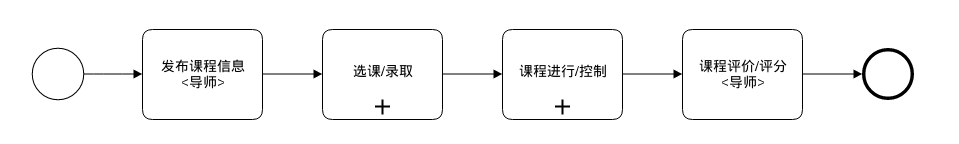
\includegraphics[scale=0.5]{figures/diagram-bpm-overview.png}
    \caption{业务过程模型示意图(概览)\label{BPMOverview}}
  \end{center}
\end{figure}

\section{小结}

在构造需求模型的过程中,维持需求的有效性、一致性、完备性、真实性和可检验性是有一定难度的,在本项目的需求模型构造过程中通过维持需求-目标的可追溯性来保持这些性质。

\begin{figure}[!hbp]
  \begin{center}
    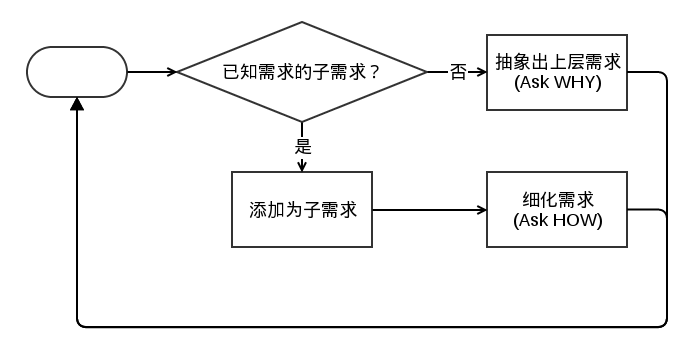
\includegraphics[scale=0.5]{figures/diagram-requirement-workflow.png}
    \caption{需求发现-验证流程(构造可追溯的需求)\label{RequirementExtraction}}
  \end{center}
\end{figure}

在与系统客户讨论和确定需求的过程中,业务过程模型发挥着很大的作用,通过与系统客户在系统业务上达成共识能够很快的发现与业务相关的功能性需求。

需求分析是软件项目开发中非常重要的环节,需求分析的过程中所产生需求文档在沟通过程中能够发挥巨大的作用。在文档中恰当的使用各类图形化的表达方法也有助于对系统中重要需求的理解与发现。

下一章将叙述从产品需求出发进行系统概要设计的过程,与需求的构造模式相似,概要设计内部以及概要设计与需求之间保持着可追溯的关系。

